\begin{wrapfigure}{r}{7.5cm}
		\vspace{-2em}
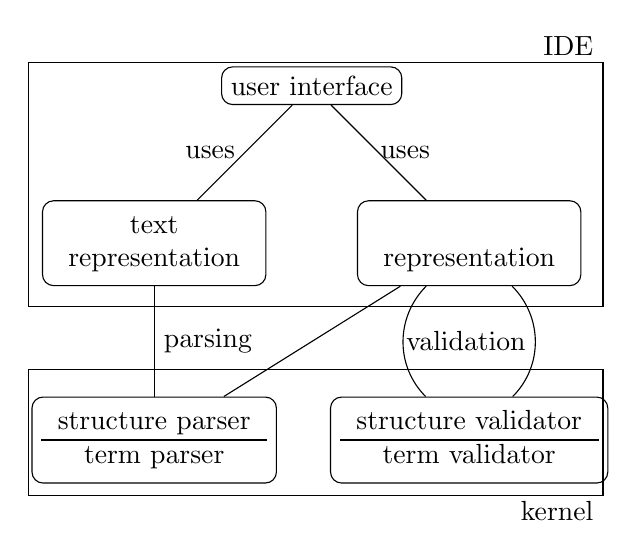
\begin{tikzpicture}[data/.style={rectangle,draw=black,rounded corners}]
  \node[data] (U) at (-2,4) {user interface};
  \node[data] (T) at (-4,2) {\begin{tabular}{c}text \\ representation\end{tabular}};
  \node[data] (M) at (0,2) {\begin{tabular}{c}\mmt\\ representation\end{tabular}};
  \draw (-5.6,1.2) rectangle (1.7,4.3) node[above=0.2cm,left] {\jmmt IDE};
  \node[data] (p) at (-4,-0.5) {\begin{tabular}{c}structure parser \\ \hline term parser\end{tabular}};
  \node[data] (v) at (0,-0.5) {\begin{tabular}{c}structure validator \\ \hline term validator\end{tabular}};
  \draw (-5.6,-1.2) rectangle (1.7,0.4) node[below=1.8cm,left] {kernel};
\draw[-\arrowtip] (T) --node[right] {parsing} (p);
  \draw[-\arrowtip] (p) -- (M);
  \draw[-\arrowtip] (M) to[out=-135,in=135] (v);
  \draw[-\arrowtip] (v) to[out=45,in=-45] node[left] {validation} (M);
\draw[-\arrowtip] (U) --node[left] {uses} (T);
  \draw[-\arrowtip] (U) --node[right=-.1cm] {uses} (M);
\end{tikzpicture}
	\vspace{-2em}
\end{wrapfigure}

An \textbf{overview} of architecture is shown on the right, where the abstraction layer separates \jmmt from a kernel.
Both the concrete text source and its abstract \mmt representation are maintained and used by \jmmt.
\jmmt uses abstract operations for parsing and validation, which are provided by kernels.

\begin{wrapfigure}{r}{7cm}
	\vspace{-2.5em}
	\begin{tabular}{|l||ll|}
		\hline
		 operations & Parsing & Validation \\
		\hline
		\hline
		Structure & Sect.~\ref{sec:sp} & Sect.~\ref{sec:sv} \\
		Terms     & Sect.~\ref{sec:tp} & Sect.~\ref{sec:tv} \\
		\hline
	\end{tabular}
	\vspace{-1em}
\end{wrapfigure}



More concretely, the abstraction layer consists of the  operations shown on the right.
Along one dimension, we distinguish the \textbf{structure} and \textbf{term} levels.
The structure level comprises the names of the theory and constant declarations.
This corresponds to the OCaml toplevel in HOL Light \cite{hollight} or to the outer syntax of Isabelle.
The term level comprises the type and definiens of the constant declarations.
This corresponds to the HOL Light formula parser or to the inner syntax of Isabelle.

Along the second dimension, we distinguish \textbf{parsing} and \textbf{validation}.
The former produces an abstract syntax tree that closely resembles the source text;
the latter refines this AST using advanced operations such as type checking, theorem proving, or computation.
Notably, we use \mmt to represent both the parsed and the validated representation, i.e., validation is a transformation from \mmt syntax to \mmt syntax.




A major \textbf{motivation} of this separation is to isolate the validation of terms.
This has three reasons.
Firstly, this is the most expensive phase.
Therefore, as we described in the change management section, isolating this component permits revalidating terms as rarely as possible.
Secondly, almost all errors that users have to fix are detected during term validation, whereas the other  components succeed most of the time.
By isolating term validation, we can provide substantial UI features, which are especially helpful when term validation does not succeed.
Moreover, many UI features do not depend on term validation such as auto-completion or search.


Thirdly, it opens up an alternative way to connect an existing kernel with our UI in those cases where it is not possible to have the kernel expose the AST.
Then it can be feasible to reimplement the other  components from scratch, but it will usually be impossible to reimplement term validation.

We explain the  components in the following, using our kernel for LF as a running example.
To simplify the description below, we point out two \textbf{general aspects} globally that apply to all  components.
Firstly, to maximize \textbf{extensibility}, both individual kernels as well as extensions of our example kernel are supplied to \jmmt as plugins.
Thus, kernels can be developed and used without rebuilding \jmmt itself.

Secondly, all  components can \textbf{report errors} to \jmmt and can always recover from errors by returning partial or no results.
For example, term parsing may return a term with some unparsed sub-terms, for which errors are reported.

\subsection{Structure Parsing}\label{sec:sp}

Structure parsing takes a source document and returns an abstract syntax tree (AST) in the \mmt language.
Alternatively, the AST can be returned as XML (using the \omdoc format \cite{omdoc}), which is useful if kernels are implemented in other programming languages.
The terms occurring in the source can remain unparsed: \jmmt produces a parsing unit for each unparsed object, which is passed on to the term parsing component.

\begin{example}[A Keyword-Based Parser]
We implement a straightforward structure parser based on keywords.
First it splits a file into declarations based on a few reserved characters and computes their source references.
Then the parsing of each declaration is relegated to an appropriate plugin, which is selected based on the keyword.

We choose the ASCII characters 28-31 as separators (the green boxes in Fig.~\ref{fig:jedit}).
For entering them, we provide \jedit actions that users can bind to, e.g., any key combination.
Thus, existing term parsers can be reused easily no matter what special characters are used in the terms.

Our structure parser works at the \mmt level, and we do not have to customize it for LF at all.
\end{example}

\subsection{Structure Validation}\label{sec:sv}

Structure validation is a fixed algorithm, that implements the semantics of \mmt, in particular the module system \cite{RK:mmt:10}.
Thus, it is not necessary to change the implementation in specific kernels.

Because \mmt is parametric in the underlying type system, the terms cannot be validated generically.
Instead, structure validation produces one validation unit for each term and passes them on to the term validator.
In particular, the constant declaration  in a theory  gives rise to two validation units:
 validates the judgment , and  validates the judgment .

Even though this algorithm is fixed, it is still extensible because it implements the structure level extension mechanism we presented in \cite{HKR:extending:12}.
This is general enough to express, e.g., all toplevel declarations of Mizar (as we show in \cite{IKRU:mizar:11}) or the type definition principle of HOL systems.

\subsection{Term Parsing}\label{sec:tp}

A \textbf{parsing unit} is a tuple of
\begin{inparaenum}
	\item a string  that is to be parsed into a term,
	\item the source reference  of  (if returned by the structure parser),
	\item the theory  in which  occurs.
\end{inparaenum}
Term parsing takes as input a parsing unit and returns an \mmt term  in context .
The role of  is to declare meta-variables for unknown sub-terms that are to be found during validation.
For example, the term parser may generate a meta-variable for the omitted type of a bound variable.
More generally, meta-variables can be used to represent proof that still have be found and inserted.

In \mmt, each sub-term may carry its own source reference.
Thus, the term parsing algorithm can return fine-granular source references for all sub-terms.
The \mmt implementation makes sure that source references are ignored when programs inspect terms (e.g., to check identity or for pattern-matching), but are carried along when programs transform terms by substitution or rewriting.

\begin{example}[A Notation-Based Parser]
\jmmt includes a term parser, which uses the \mmt notations of all constants that are imported into .
It returns source references for every sub-term and inserts fresh meta-variables for omitted variable types and implicit arguments.
(An argument position is considered implicit if it is not mentioned in the notation.)

In fact, our term parser is a bit more general: It also supports notations with precedences, argument sequences, and bound variable sequences.

Our term parser works at the \mmt level, and we do not have to customize it for LF -- we only have to import the theory from Ex.~\ref{ex:lf}.
\end{example}





\subsection{Term Validation}\label{sec:tv}

A \textbf{validation unit} consists of
\begin{inparaenum}
  \item a context  (as returned by the term parser),
  \item a judgment (as in Fig.~\ref{fig:judge}) whose terms may use the free variables of .
\end{inparaenum}

A term validator takes a validation unit; it verifies the judgment and returns a substitution for the variables in , i.e., it finds the unknown parts of the term.
This has the advantage that the validated term has the same structure as the parsed term so that the UI can present both at once.
Alternatively, it may be reasonable that validation returns a whole new term, e.g., its normal form.

It is important that we validate at a per-term basis and not at a per-declaration basis.
As described above, our structure validator produces two independent validation units  and  for a declaration .
For most type theories,  implies  so that validating both seems redundant.
But this design is crucial for change management, as we have seen in Sect.~\ref{sec:moc}.

\begin{example}[A Rule-Based Validator]\label{ex:tv}
We have developed a term validator for \mmt terms.
It reconstructs the unknown variables from  by using an algorithm similar to the one of Twelf \cite{twelf}.
Moreover, type checking can be performed modulo rewriting according to user-declared equalities (which are assumed to be confluent).
This term validator is described in detail in \cite{rabe:mmttypetheory:14}.

In order to maximize reuse, we only implement certain structural rules like congruence and lookup.
We use the heads of complex terms to relegate to language-specific rules, which can be provided by other plugins.
\end{example}

\begin{example}[A Term Validator for LF]\label{ex:tvlf}
	We instantiate the term validator from Ex.~\ref{ex:tv} with LF by providing LF-specific rules.
	These are inference rules that infer the types of terms with head , , , or ; a checking rule for judgments of the form ; an equality rule for judgments of the form ; a rewrite rule to turn  into  and a rewrite rule for -reducible terms of the form .
	
	Moreover, we implement a solution rule, which is used to determine the values of the meta-variables in : It applies to judgments of the form , where  is a meta-variable from , and the  are distinct bound variables, and solves  as .
\end{example}

Notably, in terms of lines of code, the LF-specific rules from Ex.~\ref{ex:tvlf}, the generic term validator from Ex.~\ref{ex:tv}, our plugin for \jedit together with \mmt, and the whole \jedit code are roughly related like .
This indicates the potential synergies of logic-independent IDEs.
	